\documentclass[11pt,a4paper]{article}
\usepackage{graphicx}

\title{Report of Kanji Assist}
\author{Witaut Bajaryn, Aleksander Mistewicz}

\begin{document}

\maketitle
\newpage

\section{Introduction}

We both attend Japanese language classes,
and one of us has started using his phone in Japanese.
Getting meanings and pronunciations of words
is very useful in this case and helps in learning the language.

We've noticed that there are services offering translations,
but not definitions of a symbol or a group of them.
As we learn more kanji we would get help for chosen ones only.
There exist plugins that provide similar functionality, but they usually
work in a browser only.

We decided to design and implement an Android application that would
provide dictionary definition for anything that appears on a screen.

\section{Use example}

On Kanji Assist's first run the user is asked
to choose it as the currently Assitant in Settings, and the appropriate
Settings screen is shown. The user needs to allow reading screen content.

After Kanji Assist is chosen, it is ready to work.
The user can call it at any time by long-pressing the Home button.

\begin{figure}[h]
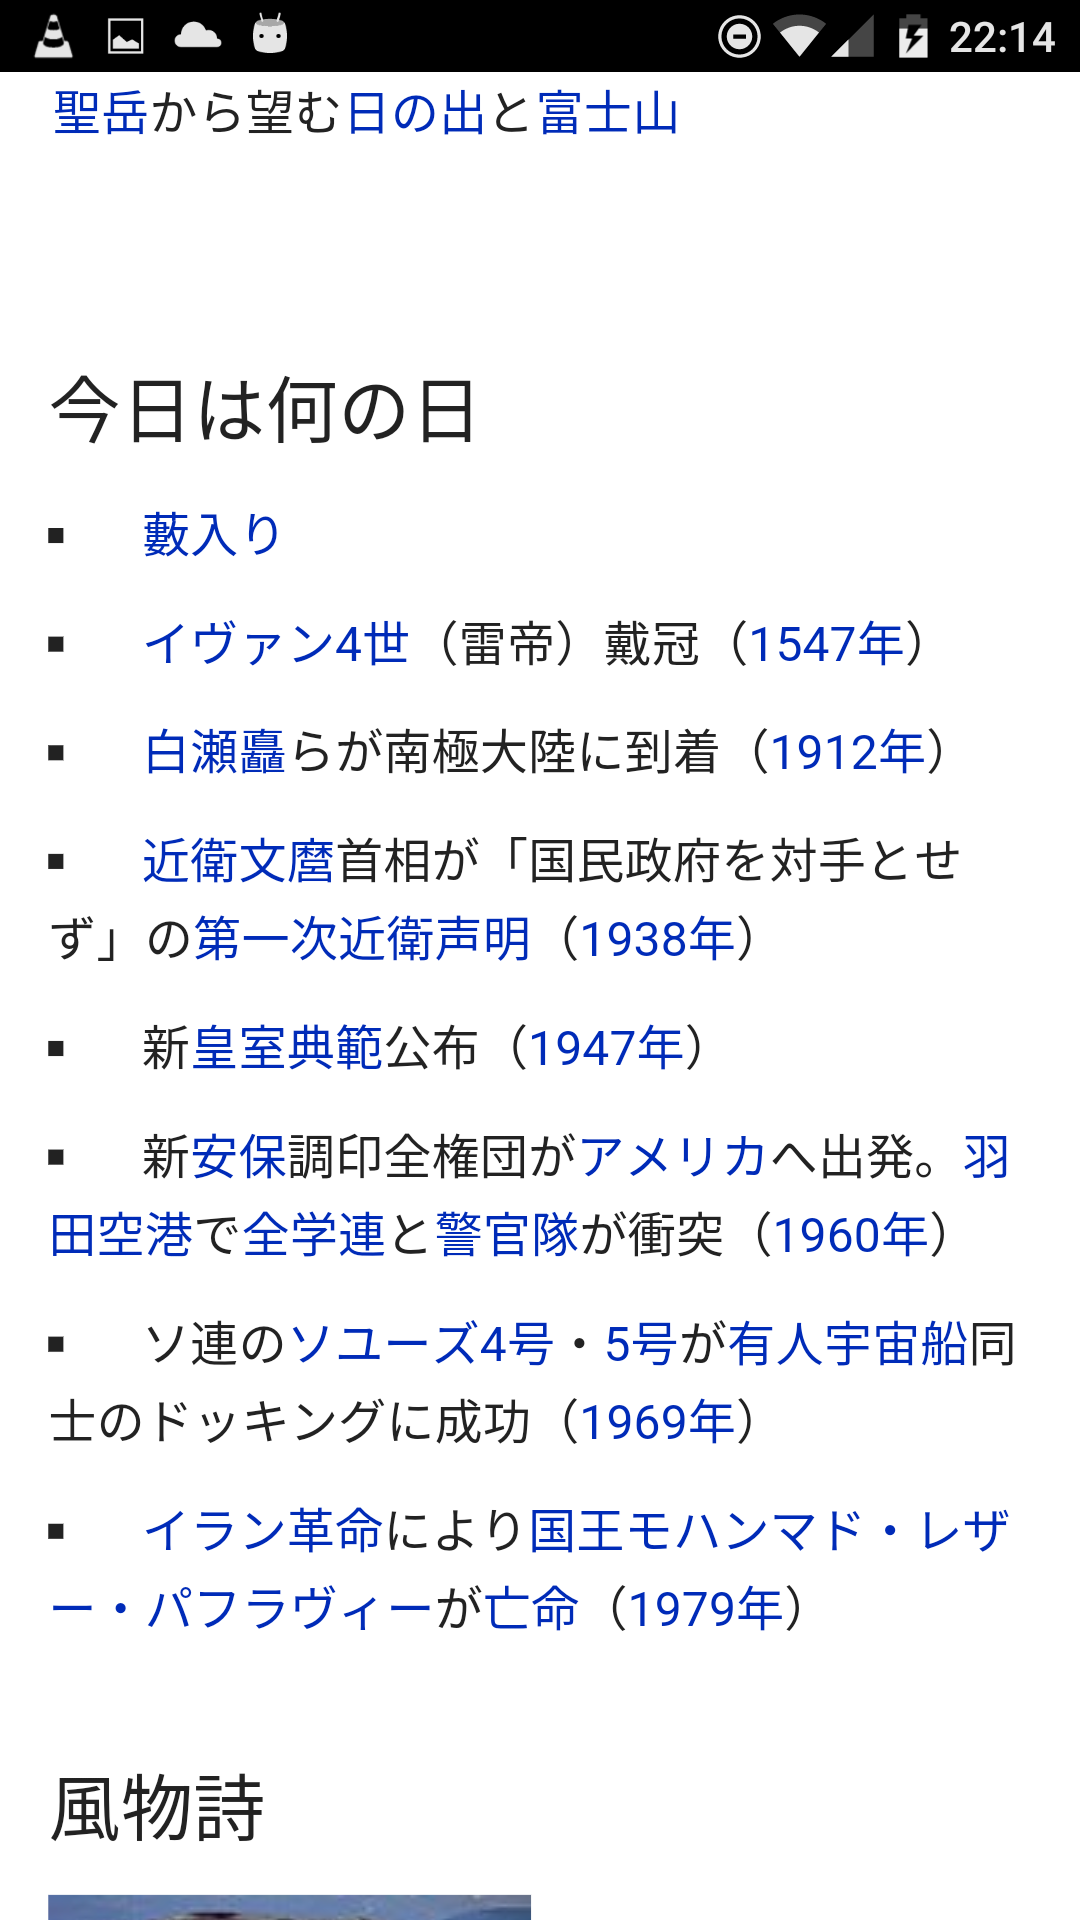
\includegraphics[width=110pt]{screen_3.png}
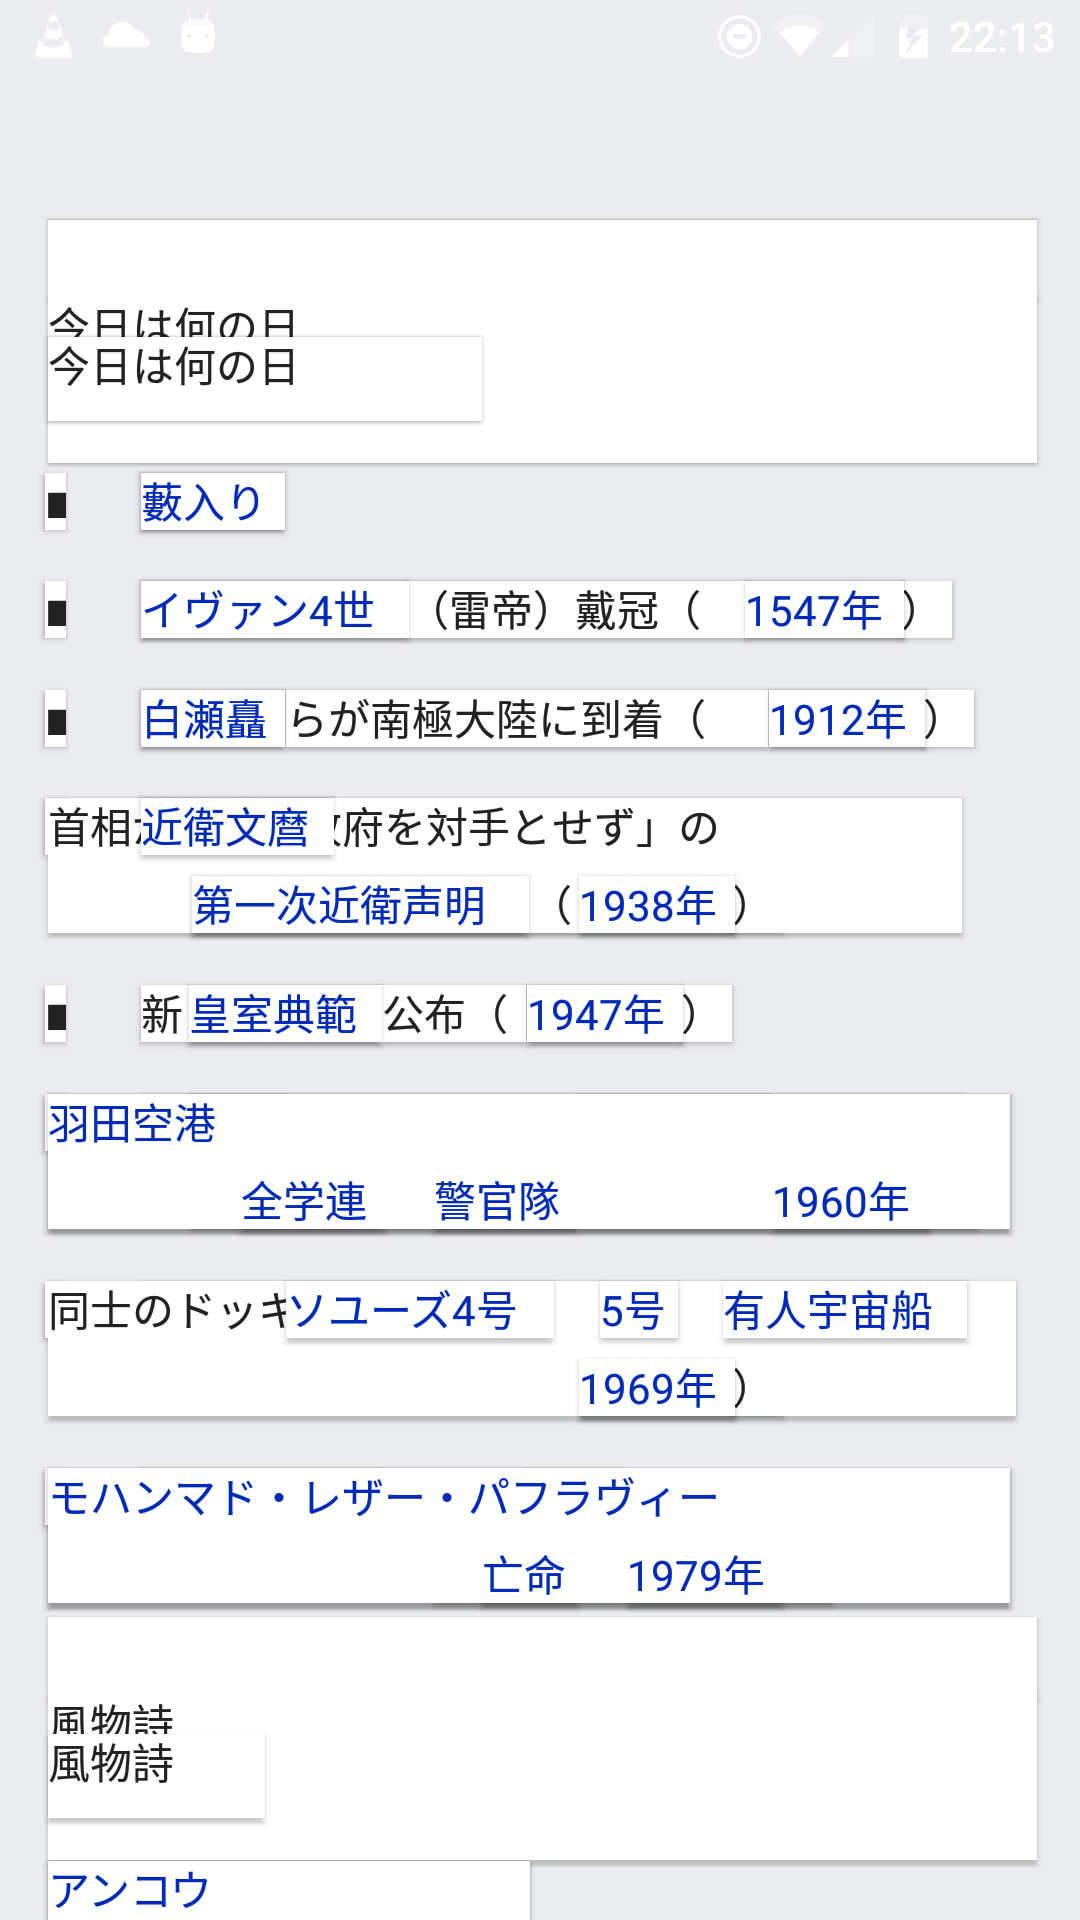
\includegraphics[width=110pt]{screen_1.png}
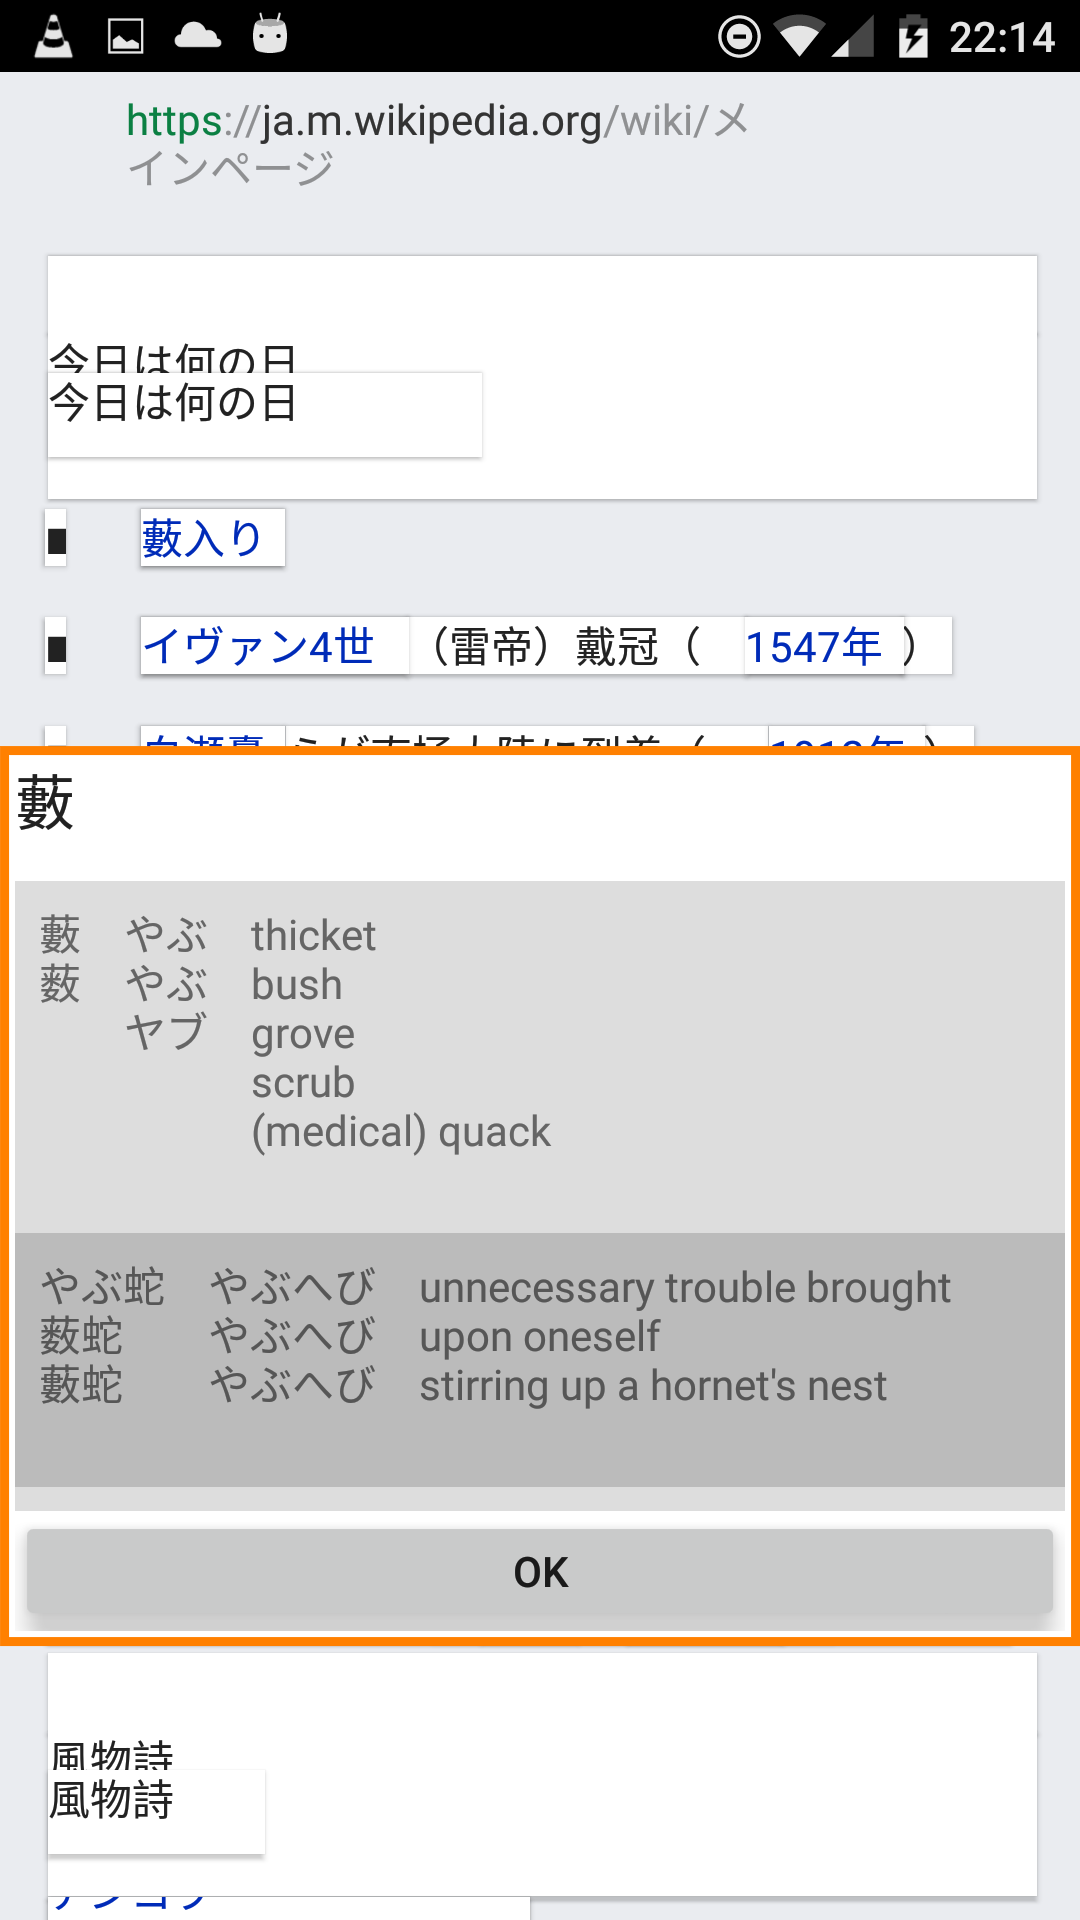
\includegraphics[width=110pt]{screen_2.png}

From the left: before calling Assistant, after Assistant's processing,
after selecting text.
\end{figure}

%The user can select some text before calling the assistant.
The text on the screen will be processed. %If any text was selected,
%a popup with its definitions and pronunciations will appear.
The user can long-press on parts of the text
or double-tap on a UI element of interest
to get a popup with information about it.
Or they can select some text before calling Assistant.

The popup contains various examples of use of the word,
and its readings and definitions in English.

\newpage

\section{Future expansion}

Our plans for the future development include:
\begin{itemize}
    \item support for different dictionaries (including a local one)
    \item dictionary prefetching
    \item user customization: themes, information displayed
    \item ability to share query with a result to another app (e.g. Anki)
\end{itemize}

\section{Problems, tests}

During the course of our work we encountered the following issues:
\begin{itemize}
    \item Android API for Asistant is almost undocumented
        and provides inconsistent data about the screen contents.

        One example is that the text size it provides
        is sometimes in pixels and sometimes in display pixels.
        The current solution to this is
        to try using it as display pixels first,
        check if it is larger than the view
        (with an unreliable way of checking)
        or than a predefined size limit (currently, 24~DP),
        and using pixels (which are usually smaller) in that case.

        Another is that some applications don't structure
        their views well (and having a flat structure is recommended
        by Google). A notorious example is Chrome,
        which makes a text view for a text block,
        and additionally a view for each hyperlink in the block,
        with no way to know which of them
        should be on top of the other --
        the views of hyperlinks
        that get wrapped around to the next line
        are as wide as the whole text block they are from.
        
    \item Assist Application implementation is not popular --
        only dummy examples available.

        The best example found was a test application
        from Android releases (6 and 7). It didn't compile,
        but removing some code that used nonexistent methods
        made it run.
    \item Most Android testing frameworks do not support Assistant testing.
    \item The user can only have one Assistant enabled at a time.
\end{itemize}

\end{document}
